%--------------------------
\subsection{Component}
%--------------------------

Formally in \mad, a component is defined as a tuple that can be divided
into four different parts: \emph{places}, \emph{transitions}, \emph{ports} and
\emph{bindings}.

\paragraph{Places}{

A component in \mad is first defined by a set of \emph{places}, denoted
$\Pi$, and two sets of \emph{docks}.  It is used to handle synchronization of parallel branches. The
first set concerns input docks. It is denoted $\Delta_{i}$
(displayed below the place they are attached to). The second set is
denoted $\Delta_{o}$. It contains output docks (displayed above
the place they are attached to).
The function $place\,:\,\Delta_{o}\cup\Delta_{i}\rightarrow\Pi$
maps docks to the place to which they are attached. Conversely, we denote by
$dock_i(\pi) \subseteq \mathcal{P}(\Delta_o)$ (respectively $dock_i \subseteq \mathcal{P}(\Delta_i)$)
the subset of output (respectively input) docks attached to a place
$\pi\in\Pi$. Places can be part of one or multiple groups which are
subsets of $\Pi$. The set of groups is denoted $G$. Last, $I \subseteq \Pi$ is the
non-empty set of initial places of the component.

}

\paragraph{Transitions}{

  % -----
\begin{table}[tp]
  \centering
  \resizebox{\columnwidth}{!}{%
    \begin{tabular}{|c|c|}
      \hline
      & \emph{Places}\\
      \hline
      $\Pi$ & set of places of a component\\
      $\Delta_{i}$ & set of input docks of a component\\
      $\Delta_{o}$ & set of output docks of a component\\
      $place$ & function mapping a dock to its place\\
      $G$ & set of groups of places\\
      $I$ & subset of places holding a token at initialization\\
      \hline
      \hline
      & \emph{Transitions}\\
      \hline
      $\Theta$ & finite set of transitions\\
      $A$ & finite set of actions\\
      $action$ & function mapping a transition to its corresponding action\\
      \hline
      \hline
      & \emph{Ports}\\
      \hline
      $S_{u}$ & set of use ports of a component\\
      $S_{p}$ & set of provide ports\\
      $T_{port}$ & set of types of ports\\
      $type_{p}$ & function mapping a port to its type\\
      $D_{u}$ & set of data use ports of a component\\
      $D_{p}$ & set of data provide ports\\
      $T_{data}$ & set of types of data ports\\
      $type_{d}$ & function mapping a data port to its type\\
      $\mathbb{D}$ & set of possible data values\\
      \hline
      \hline
      & \emph{Bindings}\\
      \hline
      $B_{S_{u}}$ & set of pairs mapping use ports to transitions\\
      $B_{S_{p}}$ & set of pairs mapping provide ports to groups of places\\
      $B_{D_{u}}$ & set of pairs mapping data use ports to transitions\\
      $B_{D_{p}}$ & set of pairs mapping data provide ports to places\\
      \hline
      \hline
      & \emph{Assembly}\\
      \hline
      $C$ & set of component instances of an assembly\\
      $L_S$ & set of use-provide connections of an assembly\\
      $L_D$ & set of data-use-provide connections of an assembly\\
      \hline
      \hline
      & \emph{Semantics}\\
      \hline
      $\mk$ & subset of elements that hold a token\\
      $\val$ & valuation function of data provide ports\\
      $\exec$ & set of ongoing actions \\
      \hline
    \end{tabular}
  }
  \caption{Defining element of the \mad formal model}
  \label{tab:not}
\end{table}
%-----
A component is also defined by a set of \emph{transitions} denoted
$\Theta$. A transition $\theta \in \Theta$ is a triple
$\left(s, \alpha, d\right)$ with $s\in\Delta_{o}$ an output dock,
$d\in\Delta_{i}$ an input dock, and $\alpha \in A$ the action
associated to the transition, taken from the set of actions $A$.
}

\paragraph{Ports}{

Places and transitions are internal elements of a \mad component.
The external interface of a component in \mad is
composed of \emph{ports}. A component contains a set of \emph{use-ports}
denoted $S_{u}$, and a set of \emph{provide-ports}, denoted
$S_{p}$. Each port is associated to a type in $T_{port}$, and the
function $type_{p}\,:\,S_{u}\cup S_{p}\rightarrow T_{port}$ maps the ports
to their type. 

In addition to traditional use-provide ports of component models,
\mad handles a specific use-provide abstraction for the
transfer of data values. These ports are called \emph{data-use-ports}
and \emph{data-provide-ports}. The set of data-use ports is denoted
$D_{u}$, and the set of data-provide ports is denoted
$D_{p}$. Each data port is associated to a type in $T_{data}$,
and the set of possible data values is denoted
by $\mathbb{D}$. Finally, the function $type_{d}\,:\,D_{u}\cup
D_{p}\rightarrow T_{data}$ maps data ports to their data type.
  
}

\paragraph{Bindings}{

  In a \mad component, places, groups of places and transitions can be
  bound to ports through \emph{bindings}. There are four sets of
  bindings.  First, we denote $B_{S_{u}}$ the set of pairs that maps
  one use port to one internal transitions in $\Theta$, indicating
  that this transition uses the service associated to this port:
  $\left(p,\theta\right)\,:\,p\in S_{u},\,\theta\in\Theta$. Second, we
  denote $B_{S_{p}}$ the set of pairs that maps one provide port to
  one group of places, indicating that if at least one token exists in
  the group, the port is active:
  $\left(p,g\right)\,:\,p\in S_{p},\,g\in G$. Third, we denote
  $B_{D_{u}}$ the set of pairs that maps one data use port to one
  internal transition in $\Theta$, indicating that this transition
  uses the data associated to this port:
  $\left(d,\theta\right)\,:\,d\in D_{u},\,\theta\in\Theta$. Finally,
  we denote $B_{D_{p}}$ the set of pairs that maps one data provide
  port to one place, indicating that the data associated to this port
  is available if a token is or has been in the place:
  $\left(d,\pi\right)\,:\,d\in D_{p},\,\pi\in \Pi$. One can note that
  multiple pairs can be defined for the same port.}

%--------------------------
\subsection{Assembly}
%--------------------------

An \emph{assembly} of components represents the instantiation of
components as defined in the previous section, and their connections
through their ports. In \mad an assembly is defined as a triplet
$(C, L_S, L_D)$, where $C$ is a finite set of component instances,
$L_S$ is the set of connections (links) between service use ports and
service provide ports of compatible types, and $L_D$ is the set of
connections between data-use ports and data-provide ports of
compatible types. For all the components $c_1,\dots,c_n \in C$, we
denote with a star any union of the corresponding sets, for instance
$\Pi^*=\bigcup_{i=1}^{n}\Pi_{i}$. We give a similar definition
for functions, for instance
$type_{p}^*\,:\,S_{u}^*\cup S_{p}^*\rightarrow T_{port}$. Connections
are defined as follows:

\begin{itemize}
\item $\left(u,p\right)\ \in L_S,:\,u\in S_{u}^{*},\,p\in S_{p}^{*},\,type_{p}^{*}\left(u\right)=type_{p}^{*}\left(p\right)$,
\item $\left(u,p\right)\ \in L_D,:\,u\in D_{u}^{*},\,p\in D_{p}^{*},\,type_{d}^{*}\left(u\right)=type_{d}^{*}\left(p\right)$.
\end{itemize}

%--------------------------
\subsection{Operational semantics}
\label{subsec:operational_semantics}
%--------------------------

At each moment in the execution of a \mad deployment assembly
$(C, L_S, L_D)$, the \emph{configuration} of this assembly is defined by a
tuple $\langle \mk, \val, \exec \rangle$, where

\begin{itemize}
  \item the marking $\mk \subseteq \Pi^{*} \cup
    \Delta_{i}^{*}\cup\Delta_{o}^{*}\cup\Theta^{*}$ denotes the
    elements that hold a token;
  \item the function $val\,:\,D_{P}^{*}\rightarrow \mathbb{D}\cup\left\{ \text{null}\right\}$
    denotes the current value associated to each data provide port;
  \item the set $\exec \subseteq A$ denotes the actions that are being executed.
\end{itemize}

The initial configuration of an assemble is given by $\langle I, v,
\emptyset\rangle$, where $v(x) = null$ for any $x$.

\noindent\textbf{Notations.}
\begin{itemize}
  \item For a function $f\,:\,A\rightarrow B$, we denote $f^{\prime}=f\left[a\coloneqq b\right]\,:\,A\rightarrow B$ such that:
    \begin{equation*}
      f^{\prime}\left(x\right)=\begin{cases}
      b & \text{if }x=a\\
      f\left(x\right) & \text{if }x\neq a
      \end{cases}.
    \end{equation*}
  \item We define the function $val_{A,D_p}\,:\,A\times
    D_{P}^*\rightarrow \mathbb{D}$ that returns the data value to assign to a
    given data-provide port after an action.
\end{itemize}

\noindent\textbf{Terminology.}

\begin{figure}[t]
  \begin{center}
    \includegraphics[width=0.7\columnwidth]{./images/enabled_service.pdf}

    \caption{The connection is enabled because its provide port is enabled, as all the groups it is bound to hold a token.}

    \label{fig:enabled_service}
  \end{center}
\end{figure}

\begin{figure}[t]
\begin{center}
  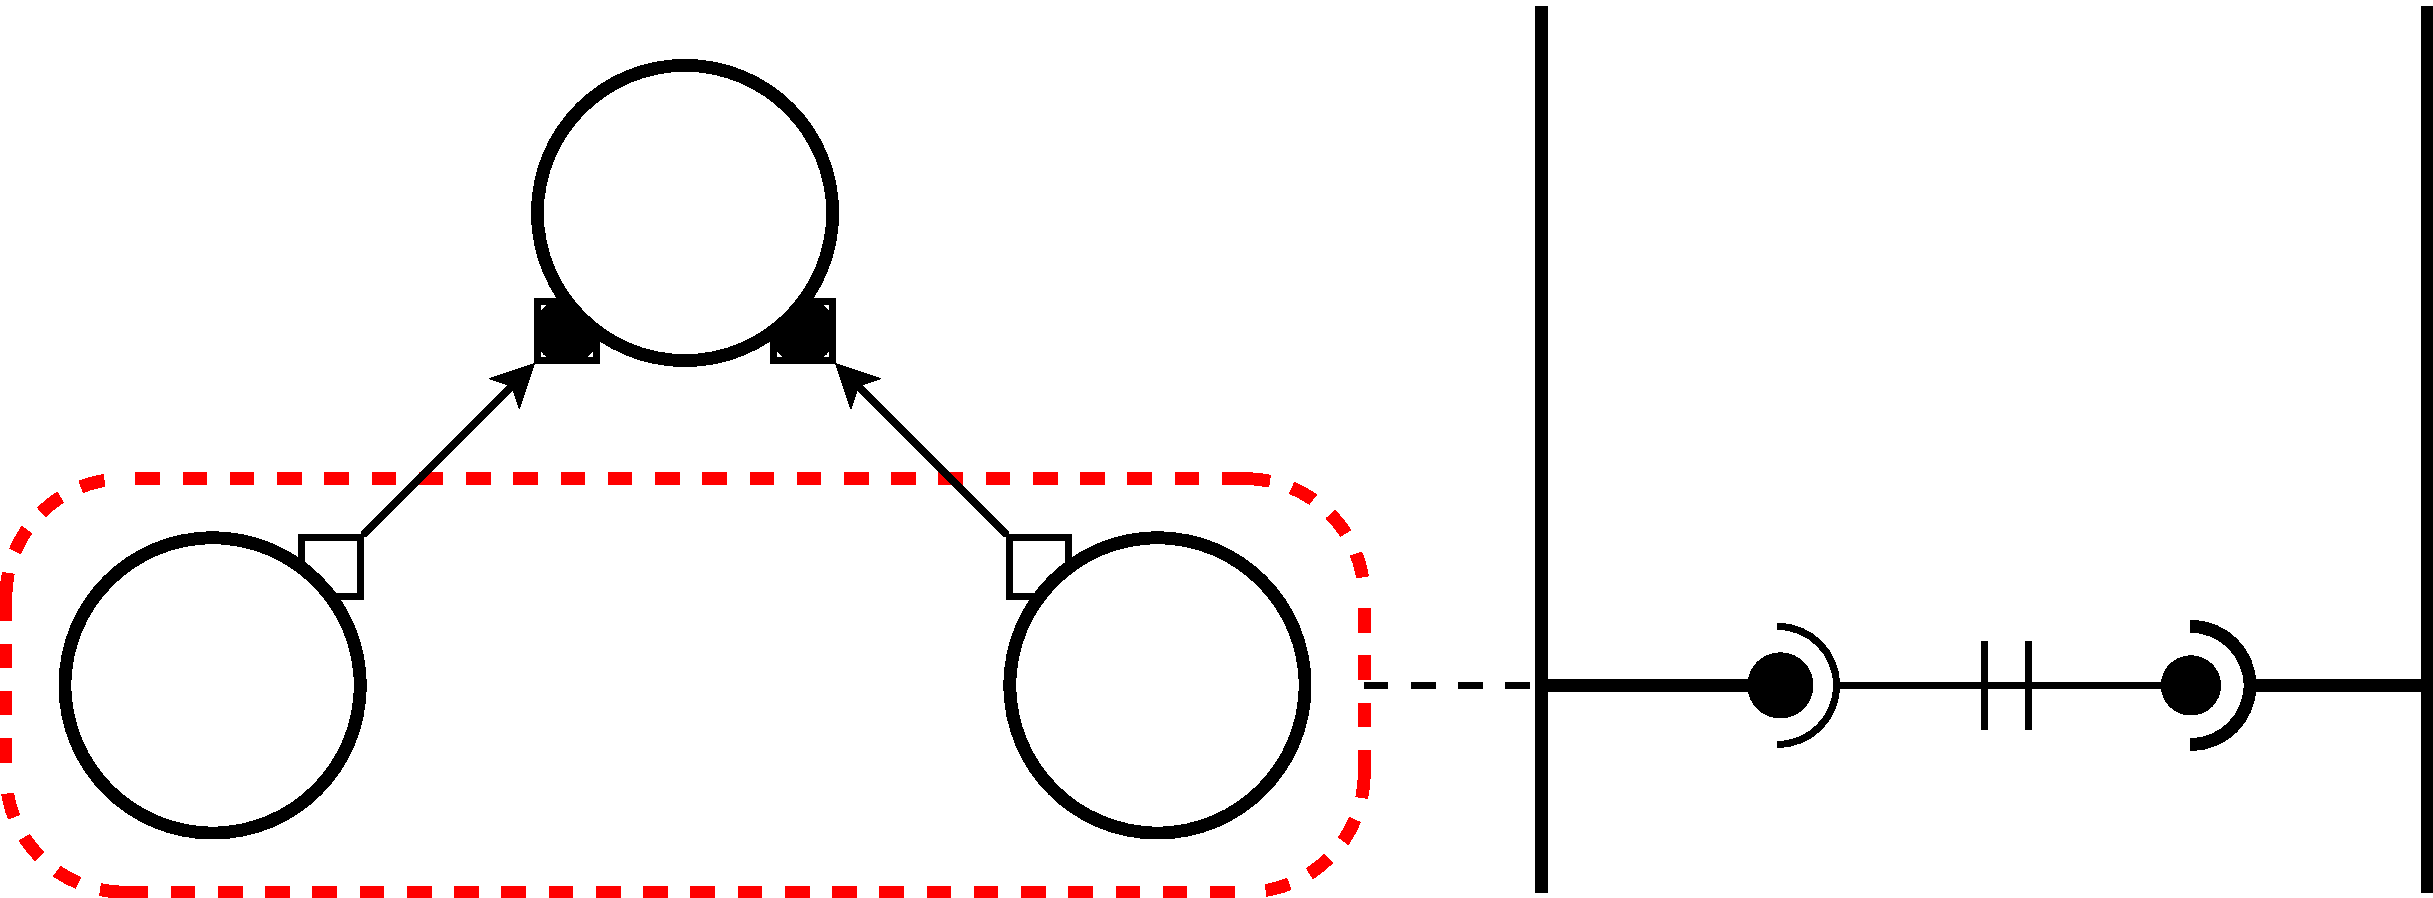
\includegraphics[width=0.7\columnwidth]{./images/disabled_service.pdf}
\end{center}
\caption{The connection is disabled because its provide port is disabled, as one of the groups it is bound to does not hold a token.}
\label{fig:disabled_service}
\end{figure}

\begin{figure}[t]
\begin{center}
  \includegraphics[width=0.4\columnwidth]{./images/enabled_data.pdf}
\end{center}
\caption{The connection is enabled because its data-provide port holds a value.}
\label{fig:enabled_data}
\end{figure}

\begin{figure}[t]
\begin{center}
  \includegraphics[width=0.4\columnwidth]{./images/disabled_data.pdf}
\end{center}
\caption{The connection is disabled because its data-provide port does not hold a value.}
\label{fig:disabled_data}
\end{figure}




A group is said to be enabled if it contains at least one token (otherwise
it is disabled). A service-provide port is said to be enabled if all the groups it
is bound to are enabled (otherwise it is disabled). A service connection is said to
be enabled if its provide port is enabled (otherwise it is disabled).
Figure~\ref{fig:enabled_service} gives an example of an enabled service connection,
while Figure~\ref{fig:disabled_service} gives an example of a disabled service connection.

A data-provide port is said to be enabled if it holds a value (otherwise it is disabled).
A data connection is said to be enabled if its provide port is enabled (otherwise it is
disabled).
Figure~\ref{fig:enabled_data} gives an example of an enabled data connection,
while Figure~\ref{fig:disabled_data} gives an example of a disabled data connection.
    
In this paper, we present four rules to operate the \mad model. We
leave for future work the extension of these rules to support errors
and reconfigurations. The rules are formally defined in
Figure \ref{fig:rules}.

\paragraph{Firing transition}{

The first rule of \mad is formally defined by
Inference rule~(\ref{eq:r1}). The upper part of the rule indicates the
hypotheses needed to fire a transition, \ie starting a transition,
and the lower part indicates the conclusion of the rule, \ie the configuration
changes. To fire a transition, the source dock of the transition
$\theta$ needs a token, and for any port bound to the transition
$\theta$ the connection of this port must be enabled.
The upper part of Figure~\ref{fig:r1} illustrates the
hypotheses and the lower part the conclusion of the rule.

\begin{figure}[t]
\begin{center}
  \includegraphics[width=0.55\columnwidth]{./images/firing.pdf}
\end{center}
\caption{Illustration of the rule of Inference rule~(\ref{eq:r1}) to fire transitions.}
\label{fig:r1}
\end{figure}

}

\paragraph{Ending transition}{

The second rule of \mad is formally defined by
Inference rule~(\ref{eq:r2}). To end a transition $\theta$, a token has to
be present on the transition and the action performed by the
transition must be terminated. When ending a transition, the token
is moved from this transition to its destination dock. Note that the ports bound
to the transition cannot be disconnected before applying this rule. Moreover, if
the place to which the destination dock is attached is bound to
data-provide ports, their values are replaced by those computed by the action.
For this reason, the rule uses the function
$val_{A,D_p}$. Figure~\ref{fig:r2} illustrates this rule.
%\MC{Expliquer pourquoi les ports ne peuvent pas etre deconnectes ?}

\begin{figure}[t]
\begin{center}
  \includegraphics[width=0.55\columnwidth]{./images/ending_transition.pdf}
\end{center}
\caption{Illustration of the rule of Inference rule~(\ref{eq:r2}) to end transitions.}
\label{fig:r2}
\end{figure}
  
}

\paragraph{Reaching place}{

The third rule of \mad is formally defined by
Inference rule~(\ref{eq:r3}). To move tokens from input docks of a place to
this place, all input docks must hold a token. The conclusion is to remove
all the tokens within the docks and to add one token inside the
place as illustrated in Figure~\ref{fig:r3}.

\begin{figure}[t]

\begin{minipage}[h]{0.45\columnwidth}%
  \centering
  \includegraphics[width=0.65\columnwidth]{./images/inputdocks_to_place.pdf}
  \captionof{figure}{\label{fig:r3}Illustration of the rule of Inference rule~(\ref{eq:r3}) to move tokens from input docks to a place.}
\end{minipage}
\hfill
\begin{minipage}[h]{0.45\columnwidth}%
  \centering
  \includegraphics[width=0.65\columnwidth]{./images/place_to_outputdocks.pdf}
  \captionof{figure}{\label{fig:r4}Illustration of the rule of Inference rule~(\ref{eq:r4}) to move tokens from place to output docks.}
\end{minipage}
\end{figure}

\paragraph{Leaving place}{

The fourth rule of \mad is formally defined by
Inference rule~(\ref{eq:r4}). To move a token from a place to its output
docks, a token needs to be present onto the place. Also, if the place
is part of a group which is itself bound to a used provide port,
applying the rule must not make the last token of the group leave,
otherwise this provide port becomes inactive. A provide port is said
to be used if it is connected to a use port bound to a transition
holding a token.  If these conditions are met, the token can be
removed from the place, and a token is added onto each output dock
attached to this place. This rule is illustrated in
Figure~\ref{fig:r4} in a simplified manner.

}

%------------
\begin{figure*}[tp]
%
\begin{equation}
  \cfrac{\theta = \left(s,\alpha,d\right) \in \Theta^*\qquad s \in \mk\qquad\forall \left(p,\theta\right)\in B_{S_{u}}^{*}\cup B_{D_{U}}^{*}\,:\,ready(p)}
        {\langle \mk, \val ,\exec \rangle \rightarrow \langle (\mk \setminus \{ s \}) \cup \{\theta\},\val,\exec \cup \{ \alpha \}\rangle }
\label{eq:r1}
\end{equation}
%
\begin{align*}
  \text{where: }ready(p) \equiv &\, \exists (u,p) \in L_{S}\cup L_D : enabled_c\left((u,p)\right) \\
  enabled_c\left((u,p)\right) \equiv &\, \begin{cases}
\forall g\in G,\left(p,g\right)\in B_{S_{p}}\,:\,enabled_g\left(g,\mk\right) & \text{if }\left(u,p\right)\in L_{S}\\
\val\left(p\right)\neq\text{null} & \text{if }\left(u,p\right)\in L_D
\end{cases} \\
enabled_g\left(g,\mk\right) \equiv & \left(\exists\,\pi\in g : \pi \in \mk\right)\\
 & \, \lor\left(\exists \theta = (s,\alpha,d)\in\Theta^{*}:\,\left(\theta \in \mk \lor s \in \mk \lor d \in \mk\right)\land place\left(s\right)\in g\land place\left(d\right)\in g\right)
\end{align*}
%
\begin{equation}
  \cfrac{\theta=\left(s,\alpha,d\right) \in \Theta^*\qquad \theta \in \mk\qquad \alpha \not\in \exec}
        {\left\langle \mk,\val,\exec\right\rangle \rightarrow\left\langle ((\mk \setminus \{ \theta \}) \cup \{ d \},\val\left[\forall p\in D_P^*,\text{dest}(p)\,:\, p\coloneqq \val_{A,D_p}(\alpha,p)\right],\exec\right\rangle}
\label{eq:r2}
\end{equation}
%
\begin{equation*}
  \text{where: }\text{dest}(p) = \left(p,g\right)\in B_{D_{p}}^*,place(d)\in g
\end{equation*}
%
\begin{equation}
  \cfrac{\pi\in\Pi^*\qquad D_i=dock_i(\pi)\qquad D_i \subseteq  \mk}
        {\left\langle \mk,\val,\exec\right\rangle \rightarrow\left\langle (\mk \setminus D_i) \cup \{ \pi \},\val,\exec\right\rangle }
\label{eq:r3}
\end{equation}
%
\begin{equation}
  \cfrac{\pi\in\Pi^{*}\qquad D_o=dock_o(\pi)\qquad \pi \in \mk\qquad \forall g\in G,\pi\in g:\,\text{can\_leave}\left(\pi,D_o,g\right)}
        {\left\langle \mk,\val,\exec\right\rangle \rightarrow\left\langle (\mk \setminus \{ \pi \}) \cup D_o,\val,\exec\right\rangle }
\label{eq:r4}
\end{equation}
%
\begin{align*}
\text{where: }\text{can\_leave}\left(\pi,D_o,g\right) = & \left(\exists p,(p,g)\in B_{S_p}:\,\text{is\_used}(p)\right)\implies \lnot \text{last\_token\_leaves} \left(\pi,D_o,g\right) \\
\text{is\_used}\left(p\right) = & \exists u\in S_{u}^{*},\theta\in\Theta^{*}:~\left(p,u\right)\in L_S\land \left(u,\theta\right)\in B_{S_u}^{*}\land \theta \in \mk \\
\text{last\_token\_leaves}\left(\pi,D_o,g\right) = & \left(\text{is\_group\_enabled}\left(g,\mk\right)\land\lnot \text{is\_group\_enabled} \left(g,(\mk \setminus \{ \pi \}) \cup D_o\right)\right) \\
\end{align*}
%
\caption{The four operational semantics rules of \mad.}
\label{fig:rules}
\end{figure*}
%------------

%--------------------------
%\subsection{Consistency rule}
%--------------------------
\textbf{Consistency.}

In \mad, the maximum number of tokens that can be used is the maximum
number of possible parallel branches. A token can only be created
during a branching (rule \emph{place to output docks}), where one
token is created for each output dock of the place. For this reason,
cycles are forbidden in \mad, otherwise an infinity of tokens could be
created which does not make sense within a commissioning procedure. We
plan in future work to support reconfiguration to allow cycles in very
specific settings to keep control on the tokens and their creation.
